\documentclass[10pt]{article}

\usepackage[T1]{fontenc}
\usepackage{geometry}
\usepackage{amsmath, amssymb, amsthm}
\usepackage{chemformula}
\usepackage{array} 

\title{Mathematics I - Problem Sheet I}
\author{Satvik Saha}
\date{}

\geometry{a4paper, margin=1in}
\setlength\parindent{0pt}
% \renewcommand\qedsymbol{$\blacksquare$}
\newcolumntype{L}{l@{\quad\quad}}

\begin{document}
        \par\textbf{IISER Kolkata} \hfill \textbf{Problem Sheet I}
        \vspace{3pt}
        \hrule
        \vspace{3pt}
        \begin{center}
                \LARGE{\textbf{CH1101 : Elements of Chemistry}}
        \end{center}
        \vspace{3pt}
        \hrule
        \vspace{3pt}
        Satvik Saha, \texttt{19MS154}\hfill\today
        \vspace{20pt}

        \begin{enumerate}
                \item Listing the elements in ascending order of atomic weights, we observe a periodicity of $5$ (with some gaps)
                        in their physical states, electrical conductivities and chemical reactivities.
                        \begin{align*}
                        \begin{array}{L L L L L}
                                \ch{Bh^2}       &       \ch{Ik^5}       &       \ch{Uc^6}       &       \ch{Dt^8}       &       \ch{Bc^{11}} \\
                                \ch{Ai^{14}}    &       \ch{Ye^{15}}    &       \ch{Sk^{17}}    &       \ch{\textbf X^{\textasciitilde19}}     &       \ch{On^{20}} \\
                                \ch{\textbf E^{23}}     &       \ch{Zw^{28}}    &       \ch{Dr^{30}}    &       \ch{Fq^{32}}    &       \ch{Fn^{36}}
                        \end{array}
                        \end{align*}

                        We may conclude that the element \ch{E^{23}} may be a gas with very low electrical conductivity and very low chemical reactivity.

                        Similarly, we may predict the existence of a new element \ch{X} having an atomic weight in the range $17-20$,
                        which may be a hard, high melting solid with very high electrical conductivity and high chemical reactivity.
                \item We will use the relation $V_m = M / \rho$ between the the molar volume $V_m$, the molar mass $M$ and the density $\rho$.
                \begin{center}
                        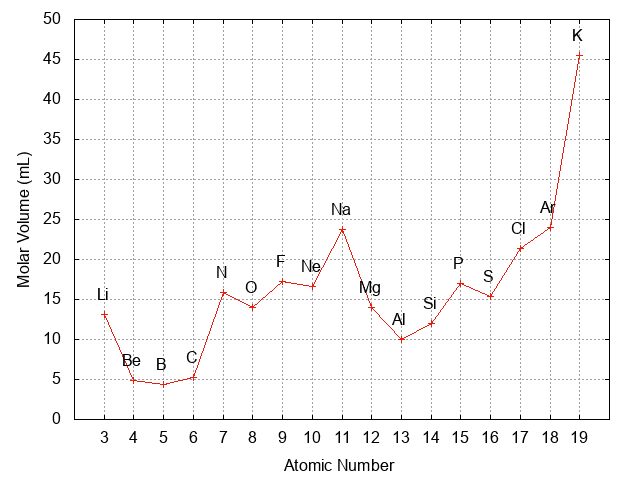
\includegraphics[scale=0.7]{volumeplot.png}
                \end{center}
                We observe that the molar volume has a general upward trend. It peaks sharply at \ch{Li}, \ch{Na}, \ch{K} (Group 1),
                and has valleys at \ch{B}, \ch{Al} (Group 3).
                \item
                The power of Mendeleev's periodic table lies in its predictive nature. Seeing the gaps in his table, Mendeleev predicted the
                existence of new elements, such as `eka-boron', `eka-aluminium' and `eka-silicon', along with their physical and chemical properties
                with stunning accuracy. He was also able to correct inaccuracies in the then known atomic weights of elements using this device.

                \item We will use $c = f\lambda$ and $E = hf$.
                        \begin{center}
                        \begin{tabular}{| c | c | c | c |}
                        \hline
                        \textbf{Frequency}      &       \textbf{Wavelength}     &       \textbf{Energy}         &       \textbf{Event}\\
                        $f$                     &       $\lambda$               &       $E$                     &               \\\hline
                        $3.8 \times 10^{14}$ Hz & $7.9 \times 10^{-7}$ m        & $2.5 \times 10^{-19}$ J       &       Heating food (infrared)\\
                        $5.0 \times 10^{14}$ Hz & $6.0 \times 10^{-7}$ m        & $3.3 \times 10^{-19}$ J       &       Reading (visible light)\\
                        $3.0 \times 10^{11}$ Hz & $1.0 \times 10^{-3}$ m        & $2.0 \times 10^{-22}$ J       &       Making popcorn (microwave)\\
                        $1.2 \times 10^{17}$ Hz & $2.5 \times 10^{-9}$ m        & $7.9 \times 10^{-17}$ J       &       Dental (X-ray)\\\hline
                        \end{tabular}
                        \end{center}

                \item We will use $\lambda = h/p$, $p = mv$.
                An \ch{O_2} molecule weighs $32 \text{ amu} \approx 5.3 \times 10^{-26} \text{ kg}$. Thus, its momentum is $2.5 \times 10^{-23}
                \text{ kg m/s}$, and its de Broglie wavelength is $2.6 \times 10^{-11} \text{m} = 26 \text{ pm}$. Clearly, this is
                a small fraction ($10.7 \text{ \%}$) of the molecular length of \ch{O_2}.

                \item A UV photon will obey the relation $E = hc/\lambda$.
                \begin{enumerate}
                        \item Each photon has an energy of $E = 4990 \text{ kJ} / N_A \approx 8.3 \times 10^{-18} \text{ J}$.
                        Thus, we have $\lambda = hc/E \approx 24 \text{ nm}$.
                        \item A $500 \text{ nm}$ photon will have an energy of $hc/\lambda \approx 4.0 \times 10^{-19} \text { J}$.
                        $21$ such photons would have an energy just exceeding that of a UV photon.
                        \item Although $25$ such photons carry a total energy more than that of a single UV photon, they cannot
                        induce mutation in a strand of DNA. This is because exactly the right amount of energy must be supplied
                        to the $\pi-$bond in a thymine base in DNA for it to break, and thus mutate. The breaking of such a bond
                        involves the absorption of the photon by an electron in a bonding molecular orbital, promoting it to an antibonding orbital.
                        Such a promotion requires just the right amount of energy -- the energy difference between the two orbitals.
                \end{enumerate}
        \end{enumerate}

\end{document}
